\chapter{Discussion}
\label{sec:Discussion}
\section{Review of Results}
% Overview of results
%% Parameters under-constrained
%% Output estimates good
There are two possible causes for the large variance in
parameter estimates. First, it could be that the particle filter is
incapable of learning the model. However, given the high quality
of BOLD estimates, this is almost certainly not the case. The other
possible explanation is that the given stimulus is not sufficiently
varied to bring out all the properties of the system. While it is
possible that this is the case, it is unlikely that any
stimulus sequence could differentiate all the parameters.
Its also extremely interesting that the histograms of parameters' mean
approach the width of the prior, even when the particle filter converges
properly to far thinner distributions. Its possible the prior
distribution is far wider than
it needs to be. Finally, the fact that \autoref{sec:VeryLongSim}, which
used randomly spaced impulses,
still had a high correlation further indicates that the parameters
are ill-defined.

Thus there is little doubt that the parameters of the BOLD model are under
constrained. While unsurprising given the sensitivity analysis by Deneux et al.,
it is a notable conclusion \cite{Deneux2006}. Other methods
that calculate a point estimate of the parameters, such as least squares
or Kalman filters (which uses the first two moments) are limited in their
capacity to estimate such parameters. While estimates of
the  BOLD signal may still be correct, the
underlying parameters and state variables cannot be described without using
a joint probability distribution function. In this sense, particle
filters represent an important step forward in BOLD parameter
estimation. Representing uncertainty with a mean
and variance is insufficient; so using a particle filter
or Bayesian estimate of the posterior is not simply an enhancement,
but a necessary precaution.

Because of the ill-defined nature of the parameters, the results
of Friston et al. may have been wider than true parameter distribution
\cite{Friston2002}. Future works that attempt to calculate parameters
of the BOLD model should be run multiple times to ensure consistency,
which most likely cannot be attained. This result is particularly
troublesome given the number of papers that use those parameters for
a prior distribution.

As the results in \autoref{sec:RealData} show, the heat maps, especially
those of mutual information, closely resembled the results of SPM. While the activation
tests were more sensitive, there were some additional false positives,
though the problem is difficult to quantify. Regions with M.I. above
$0.15$ consistently fit the FMRI data well, and simulations showed that
the particle filter performed extremely well in the face of significant
noise. In sum, the estimated BOLD output remained consistent despite
large swings in parameters.

% Pros/Cons
%% Cons
%%% Computation longer than SPM
%%% Harder to interpret
%% Pro
%%% Non-parametric
%%% Real time
%%% Full Posterior
%%% More intuitive
\section{Particle Filter Review}
The Particle Filter algorithm was originally designed for on-line parameter
estimation. For this reason, there is no guarantee of optimality or even
convergence for finite measurements. However, for the BOLD nonlinear ODE
this is less of a concern than it might first appear to be. For this
particular problem there can be no guarantee of a global minimum, and although
other techniques guarantee a local minimum, tests show that the particle
filter did converge relatively quickly \autoref{sec:VeryLongSim}.

One difficulty
with the use of a particle filter when given a finite number of measurements is finding
a good weight function $P(y_k | x_k)$. This is more important for a finite
number of measurements because $P(y_k | x_k)$ needs to converge in finite time.
In spite of this potential problem, \autoref{sec:VeryLongSim} managed
to converge in less than 500 seconds.  Given sufficient
measurements it is better to let the algorithm take longer to converge, because the
convergence will be less prone to particle deprivation. The particle filter takes longer
to run than Volterra approximation method from \autoref{sec:Background Linear Approximation};
however, it is free from the uncertainty of whether a quadratic approximation is
sufficient for the BOLD model.

The particle filter also has advantages over other estimation procedures
discussed in \autoref{sec:Prior Works}. The most important advantage is that it provides
an estimate of the posterior probability, rather than a single estimate. While researchers
often want a simple estimate of parameters, such an estimate is impossible with this particular
model. The fact that the final distribution does not need to conform to a
parametric distribution is also advantageous, given the nonlinearities in the system.
While the particle filter took a day to calculate for full brain calculations, its speed
was sufficient on a quad core machine to perform real time calculations of small regions
(approximate run time .27 seconds per voxel-measurement). Today it would be possible
 to perform real time analysis of 10 voxels on an average quad core. The algorithm also scales
well and does not require burdensome amounts of memory (approximately 11 megabytes).

%A practical benefit with the particle filter is that it is mathematically
%simple. An understanding of Bayesian statistics is all that is necessary to understand
%how the particle filter works.  Additionally very few assumptions
%are needed for the particle filter. Few assumptions  reduces the risk of those assumptions
%being violated. Fewer and more realistic assumptions also make the particle
%filter more robust to unforeseen difficulties in FMRI data.

%\section{Particle Filter Options}
%There are a large number of options available in the particle filter, that
%were of little use.
%\section{Didn't Work}
%A more subtle difference that could be made in detrending is how the percent difference
%is calculated. In this work the spline was subtracted, and then the result
%was divided by the average of the initial signal. A more correct method may be dividing
%by the spline value at that particular point. The reason for not dividing by the spline
%at that point is that it could be less stable, and in a sense the trend has already
%been removed. The difference is not particularly large though
%(dividing by 1020 rather than 1000 for instance) as long as the spline didn't have heavy swings.

%Finally, rather than adding a constant to the detrended data before
%applying the particle filter, a DC gain parameter could be added to the model. In
%tests, this could work well, however, it often did not. The problem with this
%could simply be the addition of another degree of freedom without any increase in
%the number of particles. Increasing the number of particles further though
%can be computationally intractable. Thus, while this is in a sense the correct
%solution, it is an impractical one.

%Starting with a flattened
%prior (by setting weights to be non-uniform after the initial particles have
%been drawn) was not used in the final analysis. The reason for not flattening
%the prior was a practical issue with weighting points in a
%7 dimensional joint distribution. Often differences in particle weights approached machine
%precision, meaning that the flattened prior was actually far from flat. Instead
%the distribution and results became unpredictable. This
%is quantization issue that will exist unless the prior were made to be deterministic
%or the initial number particles was raised to computationally prohibitive levels.

%Another improvement that could be made to the prior is increasing the initial variance.
%This would allow the particle filter to learn a wider range of parameters; at the cost
%of decreased convergence rate and support density. In tests, both real and simulated,
%increasing the variance tended to allow the particle filter to over-smooth
%(ex \autoref{fig:badfit_param1}). In
%essence the particle filter tended to converge to a mean where the time constants
%dominated the results by smoothing out all the peaks and troughs. The result is that
%no other parameters alter the estimated BOLD signal.
%\begin{figure}
%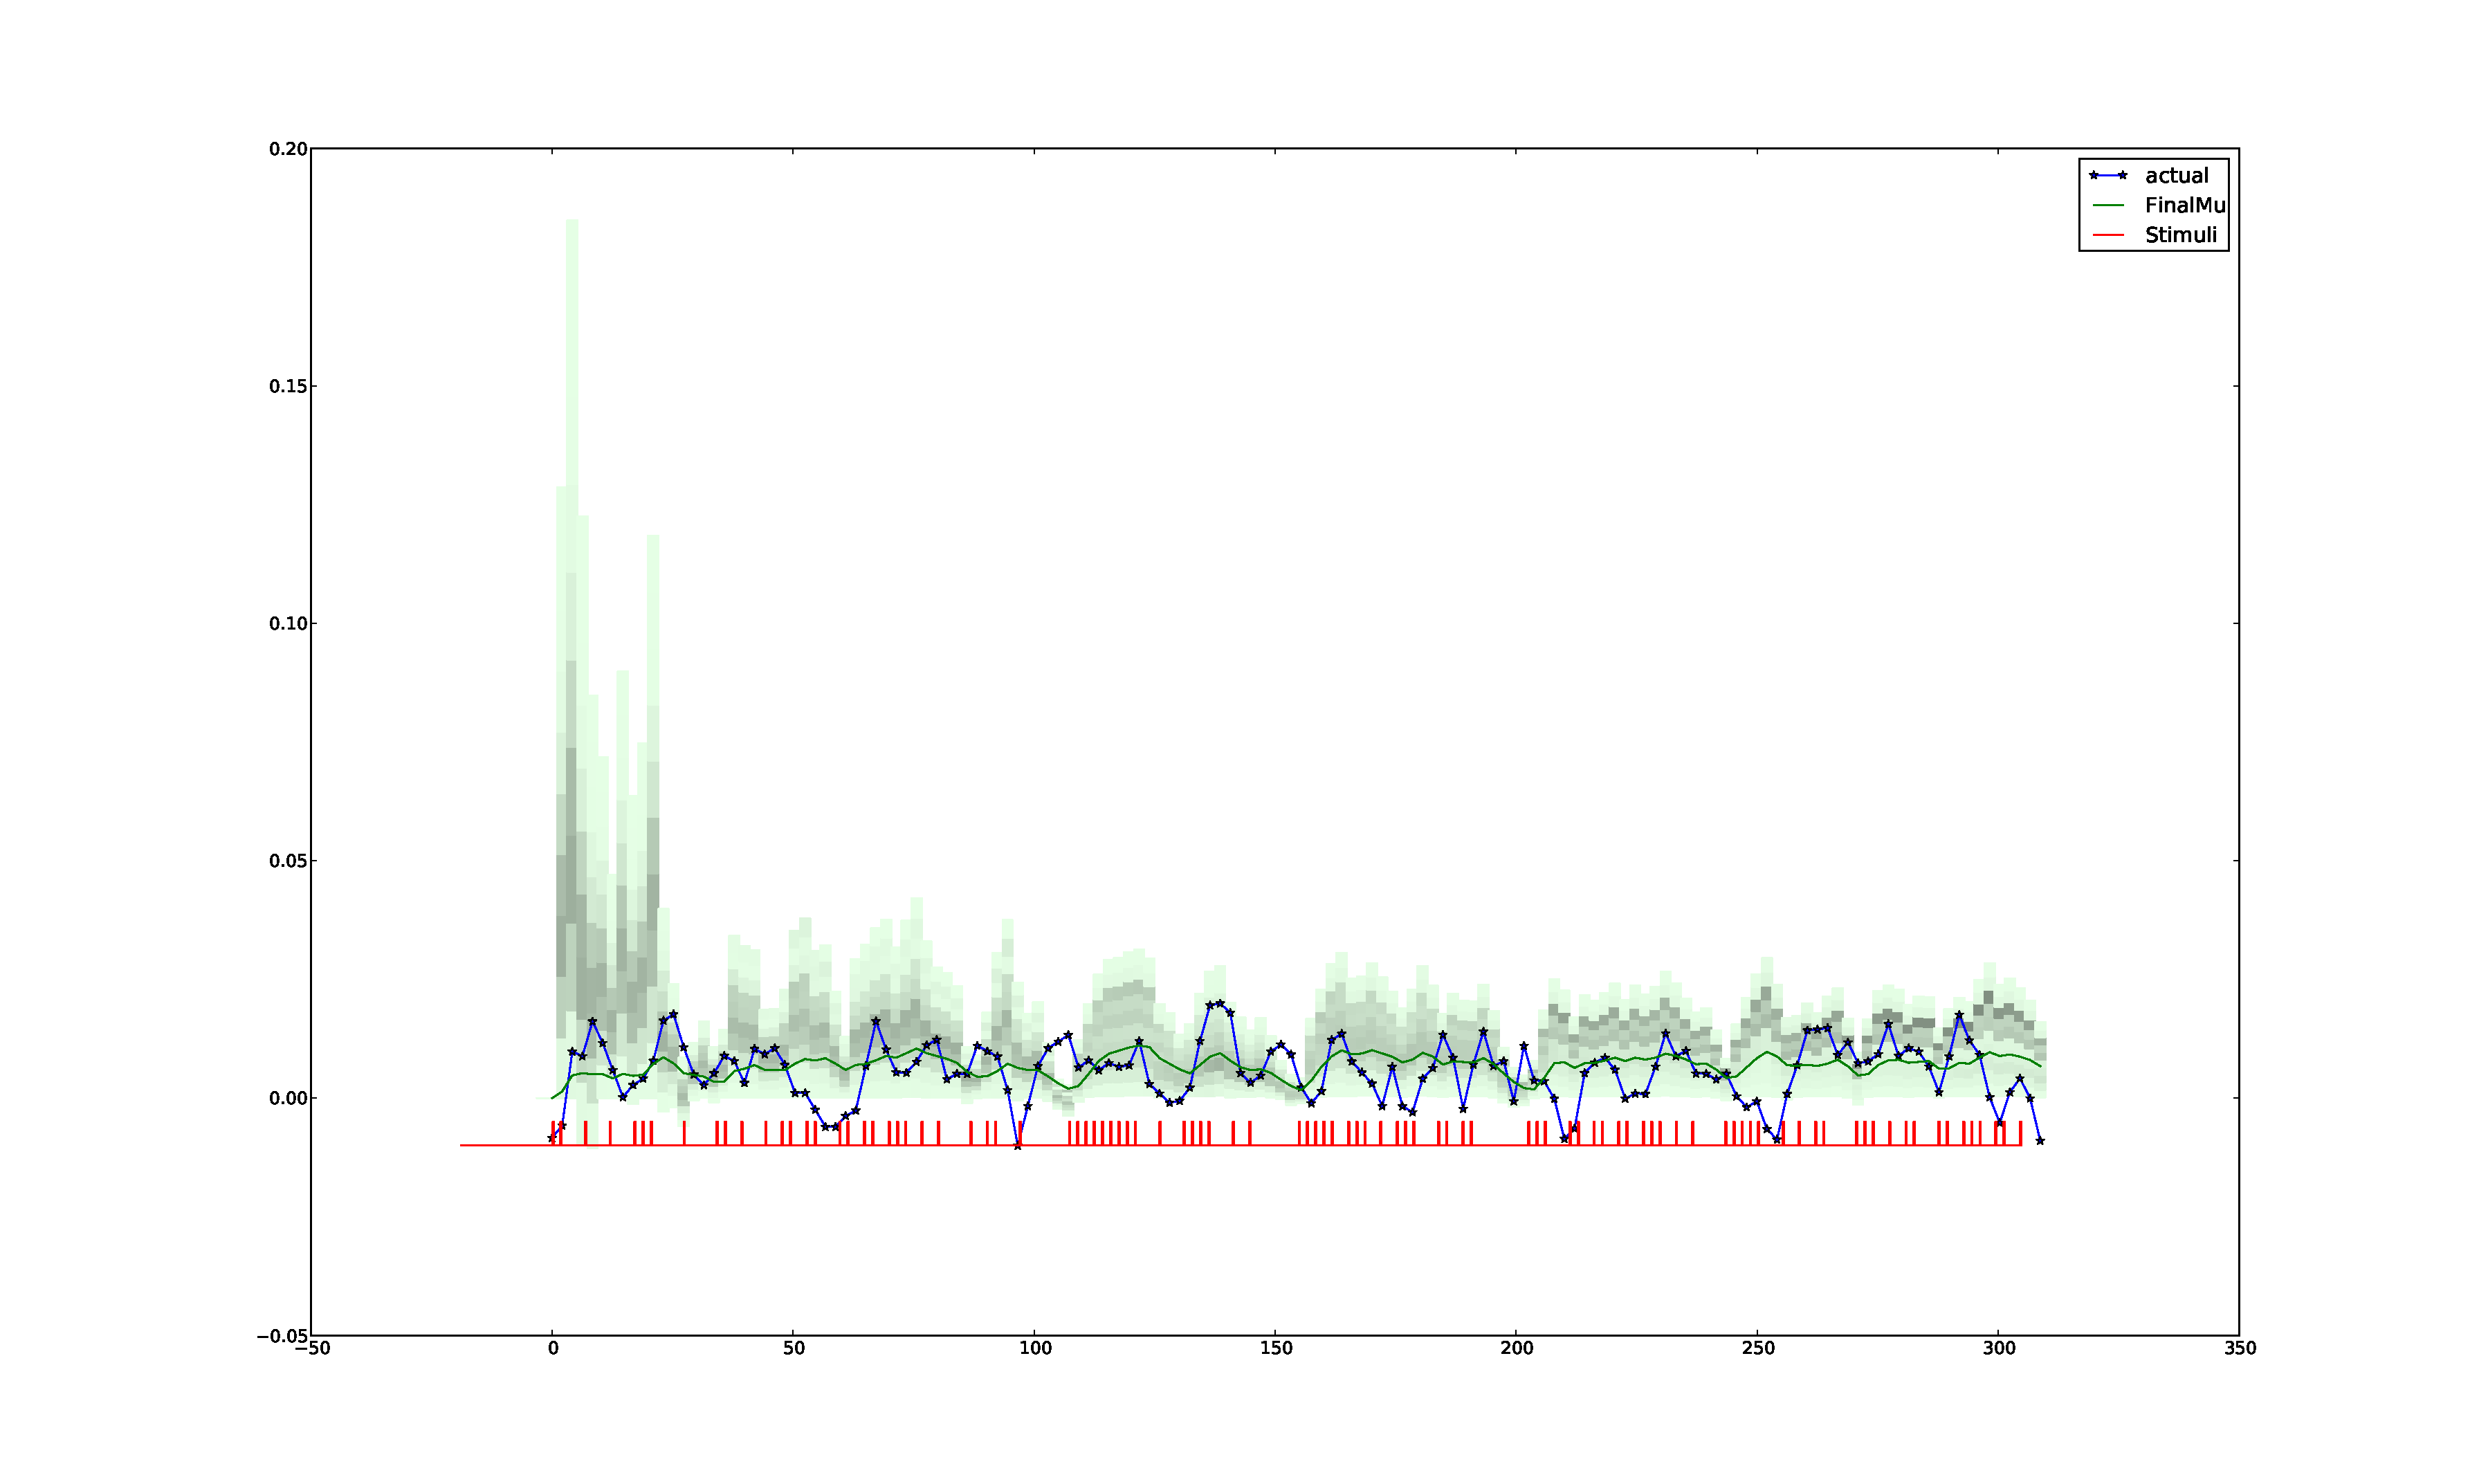
\includegraphics[clip=true,trim=6cm 2cm 6cm 3.5cm,width=7cm]{images/badfit_param1}
%\caption{Large variance in time constants over-smoothing.}
%\label{fig:badfit_param1}
%\end{figure}
%In \autoref{fig:badfit_param1}, the particle filter still had not fully converged, and
%given more measurements it could still converge to a better estimate. Thus, increases
%in the prior variance necessarily must be accompanied by more measurements,
%although re-presenting data could be used to artificially extend the measurements.

%Even more basic, its possible to artificially increase the number of
%measurements by presenting them the time-series several times.
%This activity is similar to the process used in neural networks,
%and gives the particle filter longer to converge to the optimal estimate. On the
%downside, this increases runtime and artificially reduces variance.
%Thus it does not necessarily improve the results. In tests, it did reduce the
%final covariance but did not lead to better estimates.

\chapter{Future Work}
\label{sec:FutureWork}
% Enhancements/Dehancements
%% prior
%%% flatten prior
%%% Larger variance
%% Detrending
%%% \% difference using spline?
%%% "smart knots"
%%% DC gain as a parameter
%%% linearizing
%% Experimental Changes
%%% Variations in stimuli
%%% longer timeseries or artificial
%%% Automatic estimation of measurement error.
\section{Algorithm Improvements}
\label{sec:Particle Filter Variations}
There are a few areas where future research may improve upon the current
work. The first is modifying the prior
distribution. The prior distribution used in this work is listed in \autoref{tab:Prior},
and is based on the findings of Friston et al. \cite{Friston2000}. Unfortunately, that
result depended on a quadratic approximation (Volterra Series) which has
not been extensively tested (at least not in a published work).
This is in addition to the fact that the parameters are ill-defined, and
thus the parameters found in Friston et al. are most likely far too wide.
The prior is also
based completely on the BOLD output, which is why it is good at generating
estimates of the BOLD signal, but weak at estimating parameters.
The best solution would be to have
in-vivo estimates of the actual parameters, although this
is unlikely to happen. Instead, better estimates could be found
using population studies with additional measurements as discussed in
\autoref{sec:Sideways Measurements}. Better knowledge of the prior distribution
would make it possible to decrease variance of certain
parameters, reducing the mobility of the parameters.

Another major area for improvement is removing drift.
A large number of detrending methods were tested, but every method was in some way limited.
One potentially viable method that could be utilized, given the right
experimental design, is detrending based on intervals of low activity. This
has the advantage that it wouldn't require an arbitrary
constant to be added to the pre-processed signal for the
BOLD model to fit properly. It would also minimize the actual
removed. The disadvantage of this approach is
that it could hide long fall times by normalizing them
out. It also requires periodic breaks in the stimulus,
which could reduce value of those samples for fitting purposes.

Linearizing is another possible method of dealing with drift.
This would use the delta between measurements for fitting, rather than the
direct value. This has the advantage of not requiring detrending and thus
gives nearly raw data to the particle filter for processing.
The effectiveness of this method depends directly on the type of stimulus.
In a test with rapid impulse stimuli, this could be extremely effective because
the DC signal has minimal data; conversely prolonged flat levels make this less effective.
In tests I found that large drift/low white noise
type signals performed much better with a linearization approach.
For the stimulus sequence used in \autoref{sec:RealData}, the results tended to be worse
than using spline detrending.

As discussed in \autoref{sec:Methods Weighting Function}, choosing a weighting
function is difficult, and the optimal solution varies based on the input.
Automatically estimating measurement error could improve
the quality of the particle filter results. Although I made some attempts to do
this, finding a generic, consistent solution is complex, and often depends on the
experimental design. Part of the problem is that SNR varies greatly across
the brain, and there is no way to actively measure noise without also knowing
the underlying signal. One possible solution is having the particle filter automatically
set the weight based on the total particle weight, or on the prevalence of resampling.

\section{Experimental Design Improvements}
\label{sec:Sideways Measurements}
One definite way of improving the results of the particle filter is through
additional measurements. While increasing the sample rate of FMRI scanners may
not be possible, simultaneous measurements of volume and flow is
possible, albeit at 9T in a cat \cite{Hu2009}. Just one of those measurements
would be extremely powerful when incorporated into the BOLD
model. By adding another measurement, the
variance in the parameter estimates would significantly drop. The fact
that such a measurement would be closer to the true stimulus would make it
all the more useful.
A more conventional method of adding measurements is to
simply perform longer FMRI tests. Although this wouldn't be
ground breaking, it would certainly increase the ability of the
particle filter to develop the posterior distribution.
It may also be possible to concatenate multiple FMRI tests together
by using the parameter estimates from previous tests as the
prior for later tests. 

Given the non-linearities in the system, differences in stimuli
could make a large difference in the observability of parameters. The mentality
for using a physiologically based nonlinear model for BOLD signal is to model
those nonlinearities. Its logical then that certain nonlinear parameters may not
be identifiable when the input is primarily an impulse response. It
has been reported that short responses are disproportionately large
in FMRI data \cite{Miller2001, Deneux2006}. Therefore,
a wide range of activation hold time may shed further light on
the parameters' distribution as well as the validity of the BOLD model.

% Future works
%% Using s as the input to other regions.
%% Comparison of posterior of parameters
\section{Future Applications}
There are a number of advantages to the particle filter approach presented
here. In the past, FMRI data has been analyzed strictly for determining
correlation between a stimulus and response. With this new method
the correlation is simply a means to determining the joint posterior distribution
of the parameters. While only regions that correlate with the input will
be calculable, this method exploits that correlation to constrain the
prior distribution of the parameters. The resulting distribution, while difficult
to visualize because of the high-dimensionality, could nevertheless be
correlated with neural pathologies. In spite of the fact that the parameters
are under-determined, the final distribution is still a reduction in the
uncertainty of the parameters. The availability of a full posterior distribution
opens up many avenues for further inquiry, for instance
to compare normal vs. symptomatic
populations. This would be especially useful in patients whose symptoms
are caused by functional difference in the brain, rather than structural differences.
This would effectively be
a way to differentiate the way the brains operate.

Because of limitations present in every imaging modality,
its becoming increasingly clear that combining data from multiple sources
will be necessary to push Neurology forward. In order to do so however, the
output of each source needs to fully represent what information that source
can provide. Combining the sources using Bayesian statistics is promising
yet often difficult because full probability distributions are hard to come by.
However, in this case, the particle filter provides a full posterior which
is extremely versatile. Therefore, future works will easily be able to
plug in data from multiple sources if they all output Bayesian posteriors.
For instance, if two different modalities have calculated the probability
distribution of neural efficiency, those two beliefs may be combined into
one conditional belief for a new conditional probability of neural efficiency.

An advantageous aspect of using a physiological model such as this, is that
it permits estimates of otherwise hidden parameters. In particular the BOLD
model gives an estimate of the value of the flow inducing signal, $s$. Having
this value available opens up new avenues for determining inter-regional
dependencies. The values of $s$ could serve as a proxy for activation in
that region and thus could be used to drive other inputs regions' $u(t)$.
Thus, the particle filter could be re-run
with the time-series of a particular voxel's $s$ value as an additional stimulus.
In this way, it could be possible to determine chains of events. This is just
one possible benefit being able to determine the time course of the hidden
state variables present in the BOLD equations; the potential benefits of being
able to determine this information is limitless. Of course the quality of these
estimates will continue to improve with the model priors.


